% title page

\begin{titlepage}
    \begin{center}
        \vspace{4cm}
        
        \rule{\textwidth}{1.2pt}
        
        \vspace{0.3cm}

        {\Huge \textbf{EJU PHY}}

        \vspace{0.3cm}

        {\LARGE A BRIEF SUMMARY}

        \vspace{0.3cm}

        {\Large \textit{version \version}}

        \rule{\textwidth}{1.2pt}

        \vspace{2cm}

        {\LARGE \textbf{PENG AO}}

        \vfill

        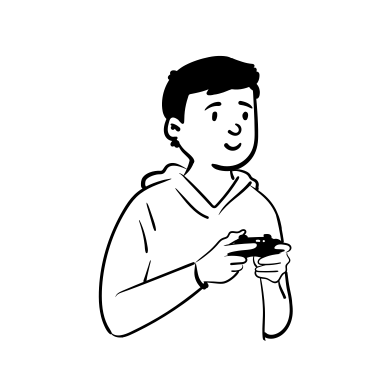
\includegraphics[width=0.4\textwidth]{avatar}

        {\Large the latest update date is \updatedate\\
        \copyright2019-22 PENG AO, All rights reserved.}
    \end{center}
\end{titlepage}

% copyright

\clearpage
\begin{flushleft}
    \null

    \vfill
    
\includegraphics{by-nc-sa}

    This work is licensed under the Creative Commons Attribution-NonCommercial-ShareAlike 4.0 International License. To view a copy of this license, visit http://creativecommons.org/licenses/by-nc-sa/4.0/.

    \vspace{1em}
    You are free to:
    \begin{itemize}
        \item Share — copy and redistribute the material in any medium or format
        \item Adapt — remix, transform, and build upon the material
    \end{itemize}

    Under the following terms:
    \begin{itemize}
        \item Attribution — You must give appropriate credit, provide a link to the license, and indicate if changes were made. You may do so in any reasonable manner, but not in any way that suggests the licensor endorses you or your use.
        \item NonCommercial — You may not use the material for commercial purposes.
        \item ShareAlike — If you remix, transform, or build upon the material, you must distribute your contributions under the same license as the original.
    \end{itemize}
\end{flushleft}

% dedication

\clearpage
\begin{center}
    \null

    \vspace{0.382\textheight}
    \textit{\large
        To my gorgeous highschool life
        and meaningful college life.
    }
\end{center}

% preface

\clearpage
\chapter*{Preface}
\addcontentsline{toc}{chapter}{前言}

本文档脱胎于2019至2021年间个人授课时所整理的大纲,主要梳理了留学生统一考试理科物理的知识点,方便教学使用。

如今2022年初,正值本人即将迈入大学\footnote{东京大学,the university of tokyo}四年级之时。出于系统练习书写\LaTeX 文档,为今后学术报告、论文撰写做准备的目的,将此前的大纲进行了重新编辑。在书写过程中尽可能采取了清晰的书写结构,力争完全使用tikz这个绘图语言包来完成文档中的插图。

文章内容参考了「わかりやすい高校物理の部屋」等网站和河合出版的《物理教室(四訂版)》等书籍,基于个人中学\footnote{东北育才外国语学校}时备考留学生统一考试时的所学所感加以补充。即便如此也难免有疏漏或是差错,欢迎在GitHub项目\footnote{https://github.com/PENG-AO/EJU-PHY}上开设Issue提出。

最后,对在教学过程中帮助我逐步做出优化调整的学生们以及编辑过程中辅助我校对的朋友们表示感谢。

\vfill
版本历史
\begin{itemize}
    \item \textit{version 1}:2019年手写版
    \item \textit{version 2}:2020年markdown电子版
    \item \textit{version 3}:2022年本文档
\end{itemize}

\vfill
\begin{flushright}
    PENG AO\\
    2022-03-30 in Tokyo
\end{flushright}

% toc

\clearpage
\tableofcontents
